\documentclass[journal,12pt,onecolumn]{IEEEtran}
\usepackage{cite}
 \usepackage{caption}
\usepackage{graphicx}
\usepackage{amsmath,amssymb,amsfonts,amsthm}
\usepackage{algorithmic}
\usepackage{graphicx}
\usepackage{textcomp}
\usepackage{xcolor}
\usepackage{txfonts}
\usepackage{listings}
\usepackage{enumitem}
\usepackage{mathtools}
\usepackage{gensymb}
\usepackage{comment}
\usepackage[breaklinks=true]{hyperref}
\usepackage{tkz-euclide} 
\usepackage{listings}
\usepackage{gvv}
\usepackage{gvv-book}
%\def\inputGnumericTable{}                                 
\usepackage[latin1]{inputenc} 
\usetikzlibrary{arrows.meta, positioning}
\usepackage{xparse}
\usepackage{color}                                            
\usepackage{array}                                            
\usepackage{longtable}                                       
\usepackage{calc}                                             
\usepackage{multirow}
\usepackage{multicol}
\usepackage{hhline}                                           
\usepackage{ifthen}                                           
\usepackage{lscape}
\usepackage{tabularx}
\usepackage{array}
\usepackage{float}

\usepackage{float}
%\newcommand{\define}{\stackrel{\triangle}{=}}
\theoremstyle{remark}
\usepackage{circuitikz}
\captionsetup{justification=centering}
\usepackage{tikz}

\title{Matrices in Geometry 1.5.25}
\author{EE25BTECH11037 - Divyansh}
\begin{document}
\vspace{3cm}
\maketitle
{\let\newpage\relax\maketitle}
\textbf{Question: }
In what ratio does the point \myvec{\frac{24}{11} \\ y} divide the line segment joining the points \textbf{P}=\myvec{2 \\ -2} and \textbf{Q}=\myvec{3 \\ 7}? Also find the value of y.\\

\textbf{Given: } 
$P\myvec{2\\-2}$, $Q\myvec{3\\7}$ and a point $R  \myvec{\frac{24}{11} \\ y}$ on $PQ$.

Let $R$ divide $PQ$ internally in the ratio $\lambda:1$.
\begin{enumerate}[label=\alph*)]
\item By section-formula,
\begin{align*}
    \myvec{\frac{24}{11} \\ y}= \dfrac{\myvec{2 \\ -2} + \lambda\myvec{3 \\ 7}}{1+\lambda}
\end{align*}

\item Cross-multiplying
\begin{align*}
    \myvec{\brak{\lambda+1}\frac{24}{11} \\ \brak{\lambda+1}y}= \myvec{2+3\lambda \\ -2-7\lambda}
\end{align*}

\item Solving for $\lambda$ and cross-multiplying, we get 
\begin{align*}
    24\lambda + 24 = 22 + 33\lambda \implies 9\lambda=2 \implies \lambda=\frac{2}{9}
\end{align*}

\item Substituting the value of $\lambda$ above, we get 
\begin{align*}
    y\brak{\frac{2}{9} +1}=-2+7\times\frac{2}{9} \implies 11y =-18+14 \implies y=\frac{-4}{11}
\end{align*}


Hence, the final answer is $\fbox{\lambda = \dfrac{2}{9}} \; \text{and} \; \fbox{y = \dfrac{-4}{11}}$


\begin{figure}[h!]
    \centering
    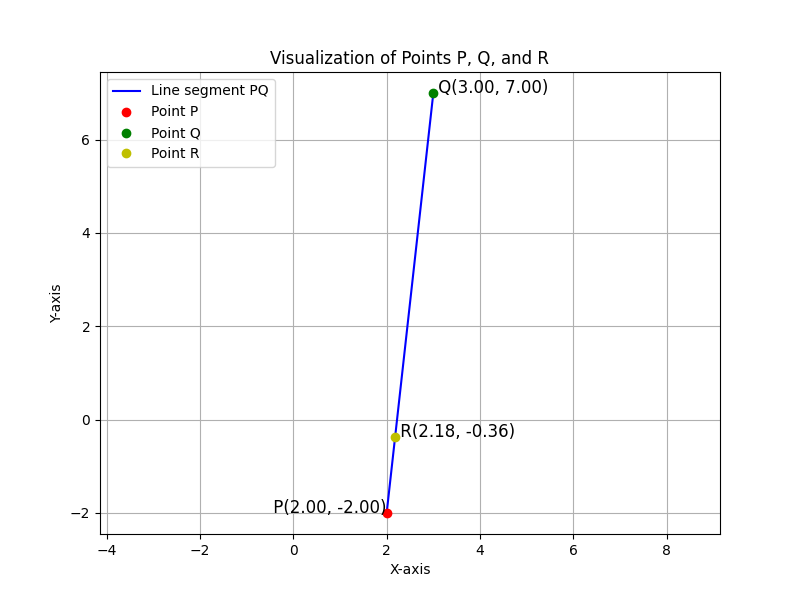
\includegraphics[width=0.5\columnwidth]{figs/1.png}
    \caption{Plot for 1.5.25}
    \label{fig:placeholder}
\end{figure}
\end{enumerate}
\end{document}